% \documentclass{lab-report}
% \usepackage{mathpazo} % Fonte MathPazo
% \usepackage{times} % Fonte Times New Roman
% \usepackage{helvet} % Fonte Helvetica
% \renewcommand{\familydefault}{\sfdefault}

% \usepackage{karnaugh-map}
% \usepackage{csvsimple}
% \usepackage{tabularray}

\documentclass[a4,12pt]{horizon-theme}
\usepackage{lipsum}
\usepackage{fontawesome5}
\usepackage{graphicx,url}
\usepackage{float}
\usepackage{amsmath}
\usepackage{booktabs}
\usepackage{makecell}
\usepackage{array}
\usepackage{multirow}
\usepackage{caption}
\usepackage{subcaption}
\usepackage{siunitx}
\usepackage{enumerate}
\usepackage{gensymb}
\usepackage{csvsimple}
% \usepackage{tabularray}
\usepackage{stackengine}
\usepackage{xcolor, colortbl}
\usepackage[round]{natbib}
\usepackage{karnaugh-map}
\usepackage{stackengine}
% \usepackage{longtable}
% \usepackage{minted}
\usepackage{fontawesome}

\strutlongstacks{T}


%%%%%%%%%%%%%%%%%%%%%%%%%%%%%%%%%%%%%%%
% Início: informações da capa
%%%%%%%%%%%%%%%%%%%%%%%%%%%%%%%%%%%%%%%
% ~~> Mudar abaixo a cada experimento <~~
% \setExpNumber{2}
% \setExpTitle{Síntese de circuito digital usando Mapa de Karnaugh}
% \setDate{29/03/2022}
% Não precisa mudar abixo
% \setTeacher{Glauber de Bona}
% \setBancada{B3}
% \setTurma{10}
% \setMemberOne{Natanael Magalhães Cardoso}{8914122}
% \setMemberTwo{Renato Naves Fleury}{11805269}
%%%%%%%%%%%%%%%%%%%%%%%%%%%%%%%%%%%%%%%%
% Fim: informações da capa
%%%%%%%%%%%%%%%%%%%%%%%%%%%%%%%%%%%%%%%%

% Cover Config
% \configCover{<num. do exp.>}{<data>}{<título>}
\configCover{2}{29/03/2022}{Síntese de circuito digital usando Mapa de Karnaugh}


% \newcommand{\n}[1]{\overline{#1}}

\begin{filecontents*}{tabelaverdade.csv}
A1,A0,B1,B0,S1,S2,S3,Z
0,0,0,0,1,0,0,1
0,0,0,1,0,0,0,0
0,0,1,0,1,1,0,1
0,0,1,1,0,1,0,1
0,1,0,0,0,0,0,0
0,1,0,1,0,0,0,0
0,1,1,0,0,1,0,1
0,1,1,1,0,1,0,1
1,0,0,0,0,0,0,0
1,0,0,1,0,0,0,0
1,0,1,0,0,1,0,1
1,0,1,1,0,0,0,0
1,1,0,0,0,0,1,1
1,1,0,1,0,0,1,1
1,1,1,0,0,0,0,0
1,1,1,1,0,1,0,1
\end{filecontents*}

\begin{filecontents*}{tabelaverdadeexp.csv}
A1,A0,B1,B0,S1,S2,S3,Z,S1_exp,S2_exp,S3_exp,Z_exp
0,0,0,0,1,0,0,1,1,0,0,1
0,0,0,1,0,0,0,0,0,0,0,0
0,0,1,0,1,1,0,1,1,1,0,1
0,0,1,1,0,1,0,1,1,0,0,1
0,1,0,0,0,0,0,0,0,0,0,0
0,1,0,1,0,0,0,0,0,0,0,0
0,1,1,0,0,1,0,1,1,0,0,1
0,1,1,1,0,1,0,1,1,1,0,1
1,0,0,0,0,0,0,0,0,0,0,0
1,0,0,1,0,0,0,0,0,0,0,0
1,0,1,0,0,1,0,1,0,1,0,1
1,0,1,1,0,0,0,0,0,0,0,0
1,1,0,0,0,0,1,1,0,0,1,1
1,1,0,1,0,0,1,1,0,0,1,1
1,1,1,0,0,0,0,0,0,0,0,0
1,1,1,1,0,1,0,1,0,1,0,1
\end{filecontents*}


%%%%%%%%%%%%%%%%%%%%%%%%%%%%%%%%%%%%%%%%
% Início do texto
%%%%%%%%%%%%%%%%%%%%%%%%%%%%%%%%%%%%%%%%
\begin{document}
\horizonCover

\horizonTitle

\section{Introdução}

Esta segunda experiência apresentará circuitos combinatórios um pouco mais complexos. Existem deiversas técnicas para a implementação desses circuitos, pois diferentes tipos de comfigurações podem dar os mesmos resultados experados. Nessa experiência será utilizada a técnica de simplificação de um circuito digital através do mapa de Karnaugh.

\section{Objetivos}
O objetivo deste projeto é explorar a técnica de síntese de um circuito a partir de sua Tabela Verdade usando Mapa de Karnaugh para gerar a expressão lógica do circuito usando um processo de montagem onde o circuito pode ser separado em componentes menores e cada componente pode ser testado individualmente.


\section{Planejamento}
No planejamento deste circuito digital, nós mostramos o processo de síntese algébrica do circuito usando Mapa de Karnaugh (Seção \ref{sec:karnaugh}), da simulação do circuito usando Quartus (Seção \ref{sec:sim}), do levantamento dos materiais necessários para construção do circuito (Seção \ref{sec:materiais}), da metodologia de montagem e teste do circuito (Seção \ref{sec:montagem}), e, por fim, consideramos possíveis alterações no planejamento que poderão ocorrer durante a construção do circuito (Seção \ref{sec:adaptacoes}).

\subsection{Síntese do circuito usando Mapa de Karnaugh}
\label{sec:karnaugh}

\begin{figure}[!ht]
\centering
\resizebox{0.6\textwidth}{!}{%
  \begin{karnaugh-map}[4][4][1][$B_1B_0$][$A_1A_0$]
  \minterms{0,2,3,6,7,10,12,13,15}
  \autoterms[0]
  \implicant{3}{6}
  \implicant{12}{13}
  \implicant{7}{15}
  \implicantedge{0}{0}{2}{2}
  \implicantedge{2}{2}{10}{10}
  \end{karnaugh-map}%
}
\caption{Resolução do Mapa de Karnaugh}
\label{fig:mapa}
\end{figure}

Primeiramente, escolhemos o nUSP de terminação $22_{10} = 0010110_{2}$ para completar as lacunas da Tabela Verdade fornecida. Com isso, montamos e resolvemos o Mapa de Karnaugh da Tabela Verdade completa, como mostrado na Fig. \ref{fig:mapa}.

% \begin{align}
%     \label{eq:karnaugh}
%     Z &= \n{A_1} \cdot \n{A_0} \cdot \n{B_0} \;+\;
%     \n{A_1} \cdot B_1 \;+\;
%     A_0 \cdot B_1 \cdot B_0 \;+\;
%     A_1 \cdot A_0 \cdot \n{B_1} \;+\;
%     \n{A_0} \cdot B_1 \cdot \n{B_0}\\
%     \label{eq:xor}
%     {} &= \n{A_1} \cdot \n{A_0} \cdot \n{B_0} \;+\;
%     \n{A_1} \cdot B_1 \;+\;
%     B_1 \cdot (\n{A_0 \oplus B_0}) \;+\;
%     A_1 \cdot A_0 \cdot \n{B_1}\\
%     \label{eq:final}
%     {} &= \underbrace{\n{A_1} \cdot (\n{A_0 + B_0} + B_1)}_{C1} \;+\;
%     \underbrace{B_1 \cdot (\n{A_0 \oplus B_0})}_{C2} \;+\;
%     \underbrace{A_1 \cdot A_0 \cdot \n{B_1}}_{C3}
% \end{align}


\begin{align}
  \label{eq:karnaugh}
  Z  & = \n{A_1} \cdot \n{A_0} \cdot \n{B_0} \;+\;
  \n{A_1} \cdot B_1 \;+\;
  A_0 \cdot B_1 \cdot B_0 \;+\;
  A_1 \cdot A_0 \cdot \n{B_1} \;+\;
  \n{A_0} \cdot B_1 \cdot \n{B_0}                    \\
  \label{eq:associativa}
  {} & = \n{A_1} \cdot \n{A_0} \cdot \n{B_0} \;+\;
  B_1 \cdot (\n{A_1} + A_0 \cdot B_0 + \n{A_0} \cdot \n{B_0}) \;+\;
  A_1 \cdot A_0 \cdot \n{B_1}                        \\
  \label{eq:xor}
  {} & = \n{A_1} \cdot \n{A_0} \cdot \n{B_0} \;+\;
  B_1 \cdot (\n{A_1} + (\n{A_0 \oplus B_0})) \;+\;
  A_1 \cdot A_0 \cdot \n{B_1}                        \\
  \label{eq:demorgan}
  {} & = \n{A_1} \cdot \n{A_0} \cdot \n{B_0} \;+\;
  B_1 \cdot (\n{A_1 \cdot (A_0 \oplus B_0)}) \;+\;
  A_1 \cdot A_0 \cdot \n{B_1}                        \\
  \label{eq:final}
  {} & = \underbrace{\n{A_1 + A_0 + B_0}}_{C1} \;+\;
  \underbrace{B_1 \cdot (\n{A_1 \cdot (A_0 \oplus B_0)})}_{C2} \;+\;
  \underbrace{A_1 \cdot A_0 \cdot \n{B_1}}_{C3}
\end{align}



A eq. \eqref{eq:karnaugh} mostra o resultado obtido ao fazer a síntese usando o Mapa de Karnaugh da Fig. \ref{fig:mapa}. A eq. \eqref{eq:associativa} mostra a redução de 5 para 3 componentes aplicando a propriedade associativa em $B_1$. A eq. \eqref{eq:xor} mostra a redução de portas lógicas para uma XOR e uma NOT. A eq. \eqref{eq:demorgan} mostra a redução de portas NOT com o uso da Lei de Morgan. E, por fim, a eq. \eqref{eq:final} mostra a expressão lógica final do circuito ao aplicar a Lei de Morgan novamente. Esta equação também indica a expressão lógica de cada um dos três componentes, que denotamos $C1$, $C2$ e $C3$.

Estas manipulações algébricas são motivadas pela busca de uma expressão lógica que satisfaça as restrições de materiais para construção do circuito físico. O processo de determinação da expressão do circuito foi feito de forma iterativa, intercalando os métodos mensionados nesta Seção e nas Seções \ref{sec:sim} e \ref{sec:materiais}. A cada manipulação algébrica da expressão lógica obtida pelo Mapa de Karnaugh, foram feitos o diagrama lógico do circuito (Seção \ref{sec:sim}) e o levantamento dos materiais necessários (Seção \ref{sec:materiais}).


\subsection{Simulação do circuito usando o Quartus}
\label{sec:sim}

\begin{figure}[!ht]
  \centering
  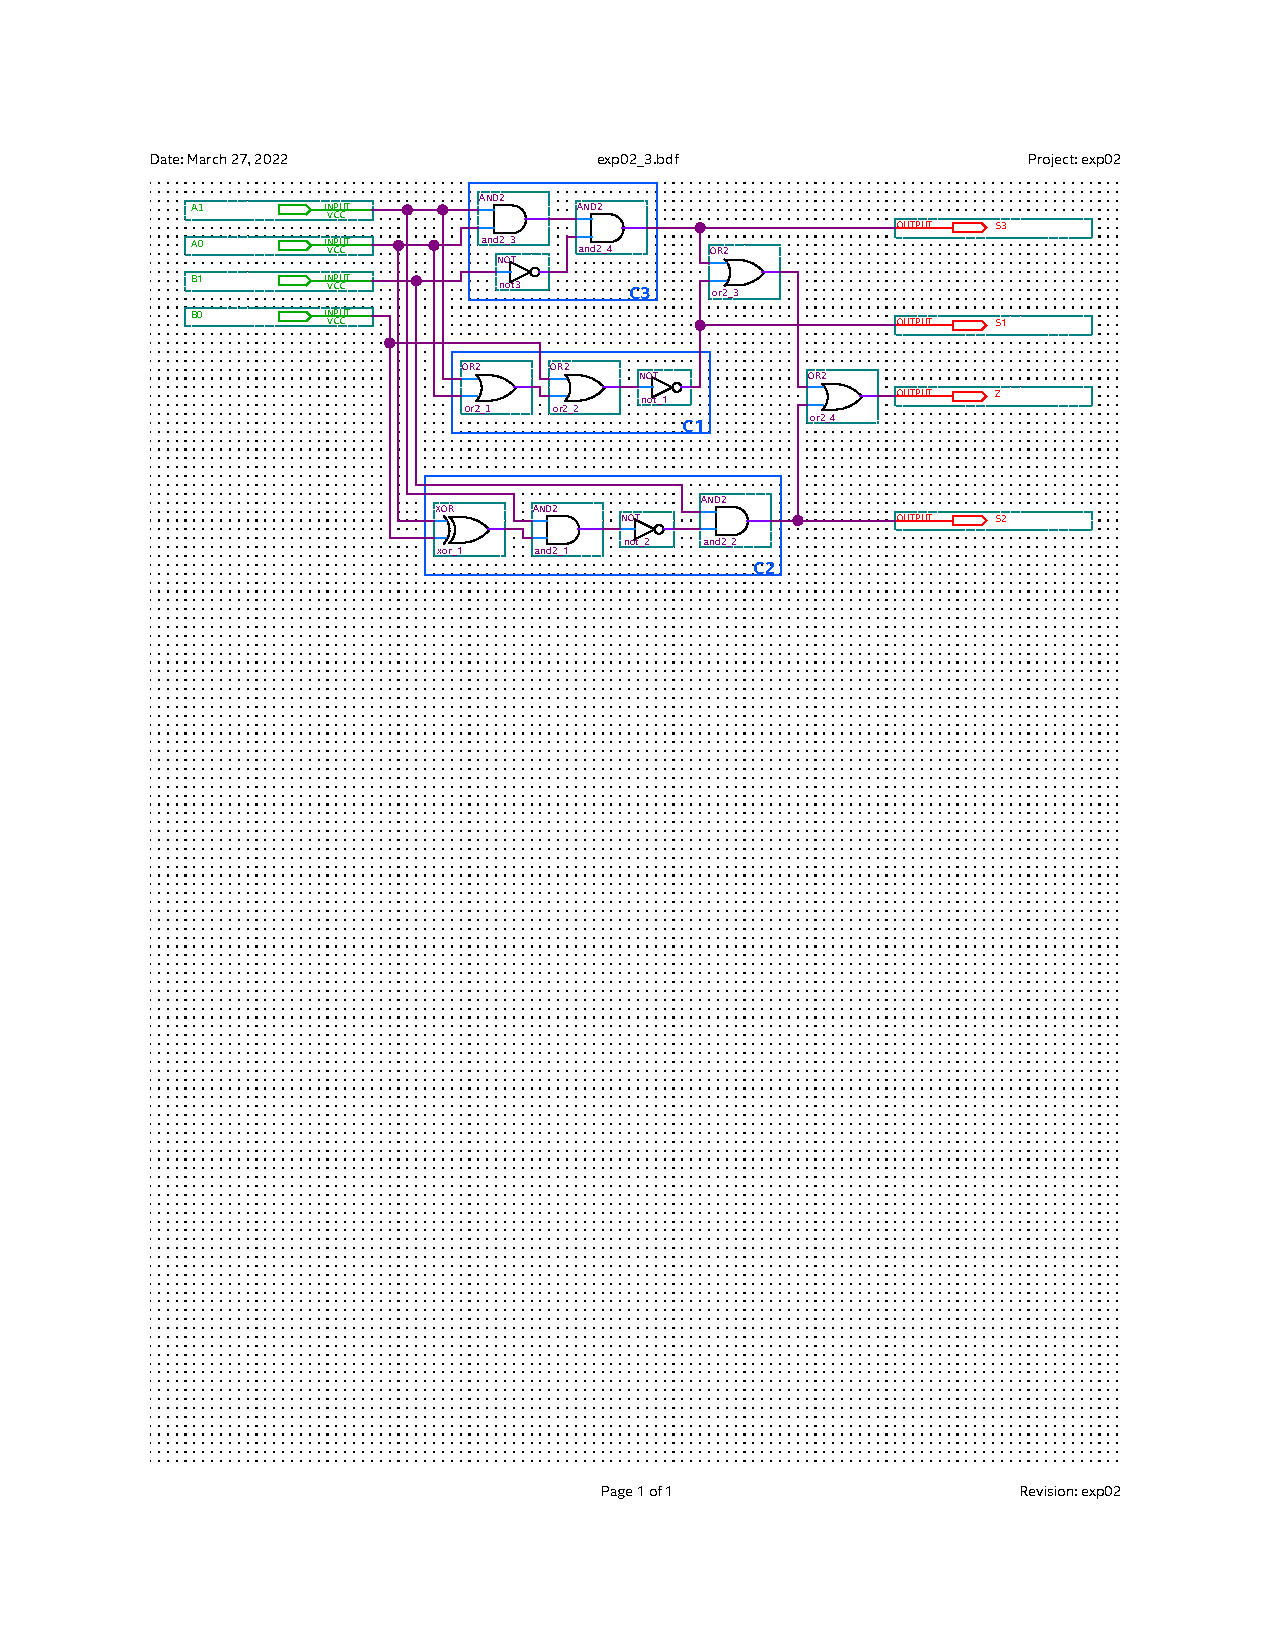
\includegraphics[width=\textwidth, trim={31mm 182mm 30mm 31mm}, clip]{diagrama_logico_v2.pdf}
  % 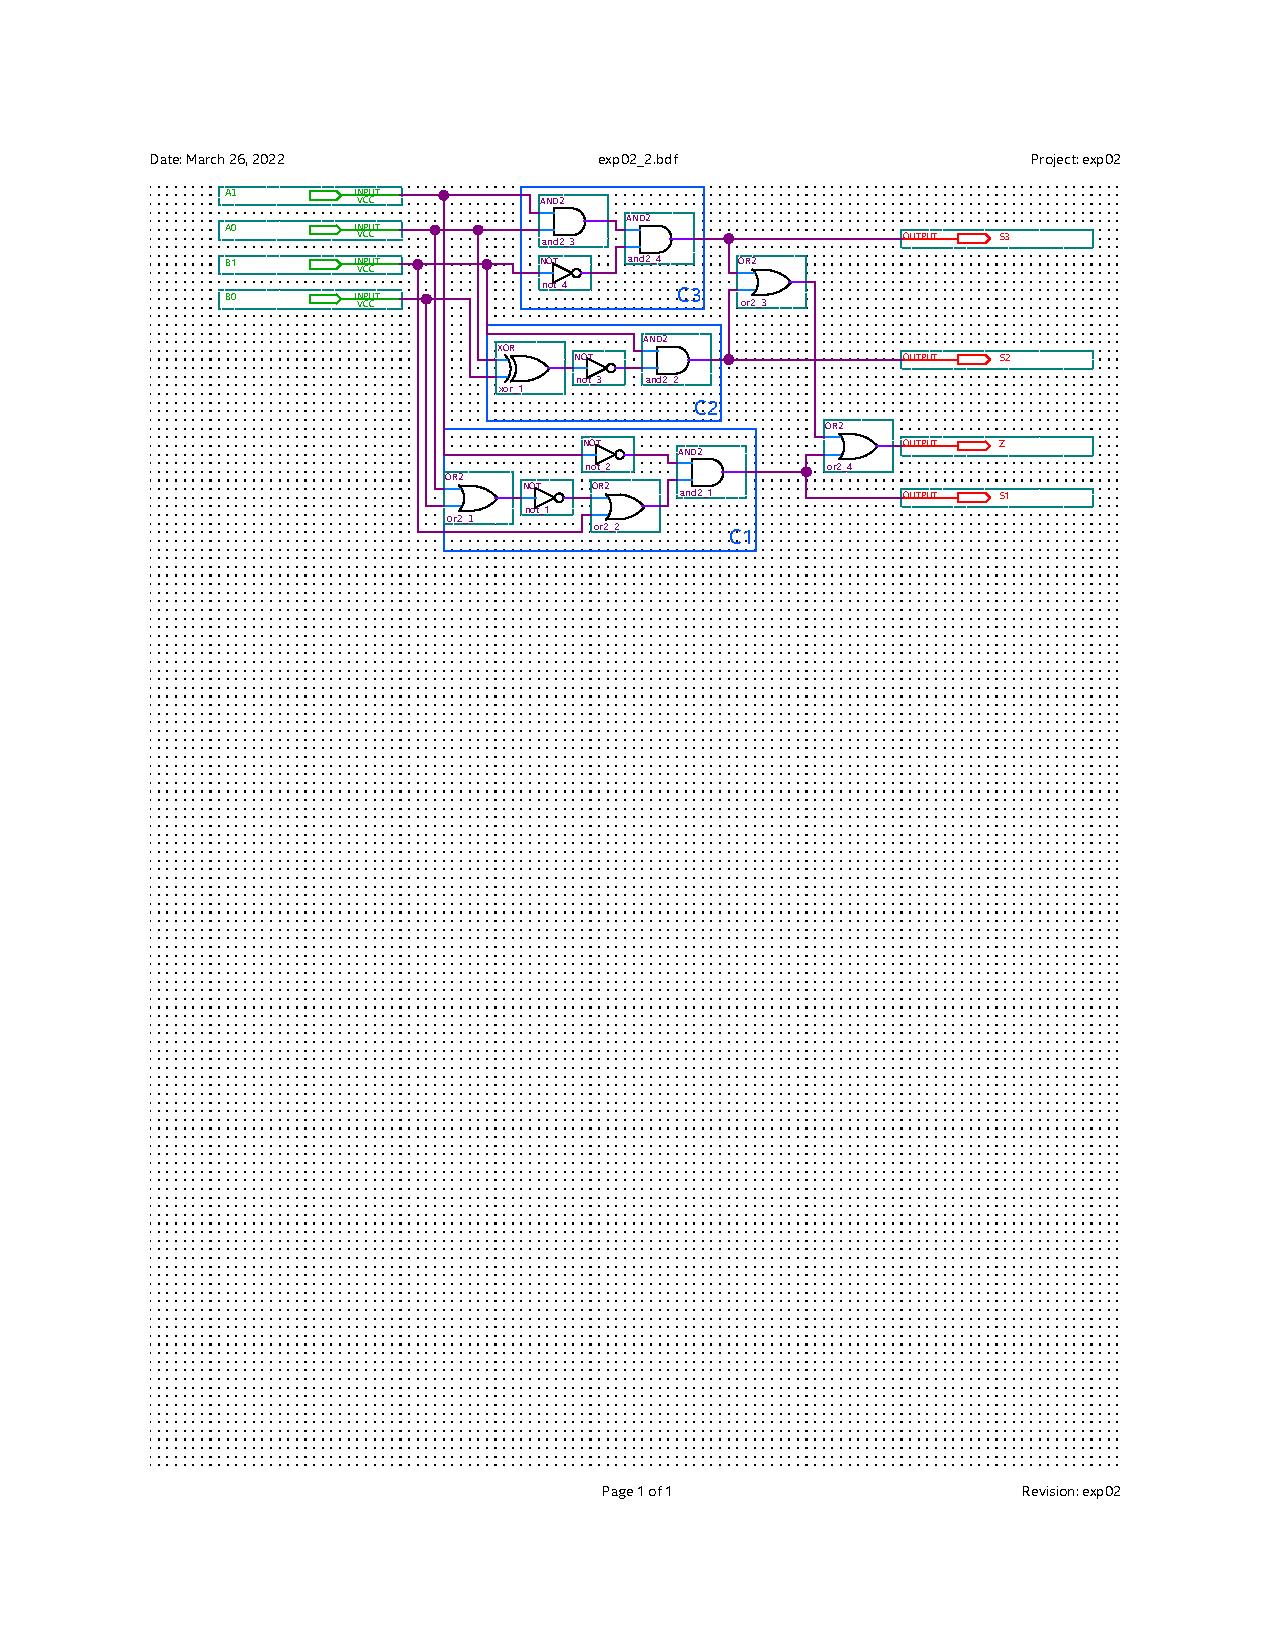
\includegraphics[width=\textwidth, trim={36mm 185mm 30mm 30mm}, clip]{diagrama_logico.pdf}
  % 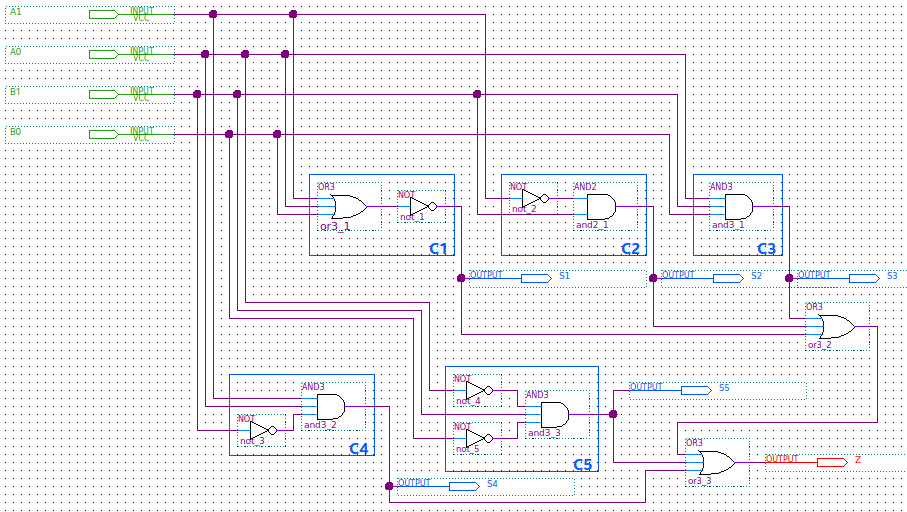
\includegraphics[width=\textwidth]{diagrama_logico.png}
  \caption[]{Diagrama lógico\footnotemark do circuito digital projetado a partir da eq. \eqref{eq:final}}
  \label{fig:diagrama_logico}
\end{figure}
\footnotetext{Imagem vetorial, é possível ampliar sem perda de qualidade.}

Ao cricar o diagrama lógico da eq. \eqref{eq:karnaugh}, percebemos que seriam necessários mais materias que os disponíveis para montar o circuito. Por isso, modificamos a expressão lógica inicial até que chegarmos na eq. \eqref{eq:final}. Com isso, obtivemos o diagrama lógico mostrado na Fig. \ref{fig:diagrama_logico}.


\begin{figure}[!ht]
  \centering
  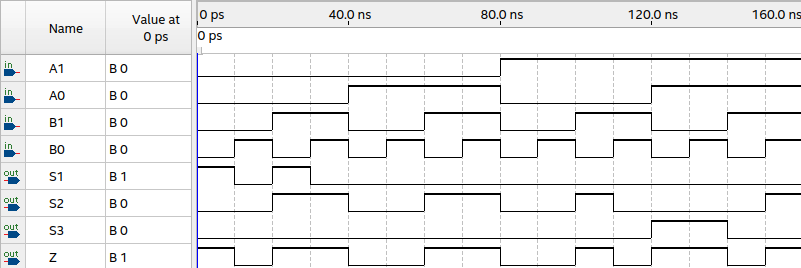
\includegraphics[width=\textwidth]{carta_tempos_v2.png}
  \caption{Carta dos tempos para o circuito simulado exibindo os sinais de entrada ordenados do mais significativo para o menos significativo ($A1$ até $B0$), os sinais intermediários ($S1$ até $S3$) e o sinal de saída $Z$}
  \label{fig:carta_tempos}
\end{figure}

Com o diagrama montado, os sinais de entrada foram configurados para que cobrissem todos os valores possíveis da Tabela Verdade. A Carta dos Tempos da simulação é mostrada na Fig. \ref{fig:carta_tempos}. A partir desta figura, foi criada uma Tabela Verdade (Tabela \ref{tab:tabela_verdade}) com os valores esperados dos sinais S1, S2, S3 e Z para cada valor de entrada.

\begin{table}[!ht]
  \centering
  \caption{Tabela Verdade dos valores esperados dos sinais intermediários $S1$, $S2$, $S3$ e de saída $Z$ para cada valor dos sinais de entrada $A_1$, $A_0$, $B_1$ e $B_0$}
  \label{tab:tabela_verdade}
  \doubleRuleSep
  \begin{tabular}{rrrrrrrr}
    \doubleTopRule
    \multicolumn{4}{c}{Entrada} & \multicolumn{4}{c}{Valor Esperado}                                                                             \\
    \cmidrule(lr){1-4}\cmidrule(lr){5-8}
    $A_1$                       & $A_0$                              & $B_1$      & $B_0$     & $S1$     & $S2$      & $S3$       & $Z$          \\
    \midrule
    \csvreader[head to column names, late after line=\\]{tabelaverdade.csv}{}%
    {\csvcoli                   & \csvcolii                          & \csvcoliii & \csvcoliv & \csvcolv & \csvcolvi & \csvcolvii & \csvcolviii} %
    \doubleBottomRule
  \end{tabular}
\end{table}


\newpage
\subsection{Levantamento dos materiais necessários}
\label{sec:materiais}

A Tabela \ref{tab:materiais} mostra a quantidade de unidades lógicas requeridas para cada CI utilizado. Isso foi feito para que a expressão lógica do circuito planejado obedeça às restrições de montagem. As especificações de cada CI foi obtido pelos respectivos \emph{datasheets}.

\begin{table}[!ht]
  \centering
  \caption{Comparação das unidades lógicas requeridas pela eq. \eqref{eq:final} e disponíveis para montagem do circuito de acordo com as características de cada CI e da placa de montagem}
  \label{tab:materiais}
  \doubleRuleSep
  \begin{tabular}{lllrr}
    \doubleTopRule
    Slot & Operação & CI   & Un. Requeridas & Un. Disponíveis \\
    \midrule
    1    & AND2     & 7408 & 4              & 4               \\
    2    & NOT      & 7404 & 3              & 6               \\
    3    & OR2      & 7432 & 4              & 4               \\
    4    & XOR      & 7486 & 1              & 4               \\
    \doubleBottomRule
  \end{tabular}
\end{table}

\subsection{Metodologia de montagem e teste do circuito}
\label{sec:montagem}

Com o circuito definido, calculamos a Tabela Verdade esperada a partir da simulação no Quartus. Para que seja possível testar cada componente separadamente durante a montagem, a Tabela \ref{tab:tabela_verdade} mostra o valor esperado da saída $Z$, bem como os valores dos sinais intermediários $S1$, $S2$ e $S3$, que são os sinais de saída dos componentes $C1$, $C2$ e $C3$, respectivamente. Estes componentes referem-se aos indicados na eq. \eqref{eq:final} e na Fig. \ref{fig:diagrama_logico}.

Visto que a Tabela \ref{tab:tabela_verdade} consta do mesmo número de sinais quanto o número de leds da placa de montagem, a ideia é montar o circuito progressivamente componente por componente e realizar uma depuração completa a cada novo componente montado na placa. No final, serão feitos quatro testes: um para cada sinal intermediário e outro para o sinal final.




\subsection{Possíveis adaptações durante a construção}
\label{sec:adaptacoes}
Embora tenhamos adotado o circuito da Fig. \ref{fig:diagrama_logico} como \emph{baseline}, não o consideramos como única opção. Adotamos este modelo por depender apenas de portas lógicas de duas entradas. Contudo, otimizações poderão ser feitas dependendo da disponibilidade de CIs durante a construção deste circuito, como a substituição de \texttt{AND2} por \texttt{AND3} e a substituição de \texttt{OR2} por \texttt{OR3}. Se todas essas mudanças forem aplicadas, haverá uma redução de três portas lógicas usadas, passando de 12 para 9.



\section{Experimento}
\label{sec:experimento}

\subsection{Montagem}

% adicionar imagem do circuito

A montagem do circuito digital foi realizada utilizando-se de uma placa de montagem, jumpers e dos CIs TTL 7404, 7408, 7432 e 7486. A Figura \ref{fig:montagem} mostra a montagem final do circuito.

\subsection{Resultado}

Com o circuto montado, testou-se todas as combinações de entrada e analisou-se as respectivas saídas comparando-as com o resultado esperado. Dessa observação obteve-se a seguinte tabela, na qual todos os sinais experimentais condizem com os resultados esperados. A Tabela \ref{tab:tabela_verdade_exp} mostra essa relação.

\begin{table}[!ht]
  \centering
  \caption{Tabela Verdade dos valores esperados e experimentais dos sinais intermediários $S1$, $S2$, $S3$ e de saída $Z$ para cada valor dos sinais de entrada $A_1$, $A_0$, $B_1$ e $B_0$}
  \label{tab:tabela_verdade_exp}
  \doubleRuleSep
  \begin{tabular}{rrrrrrrrrrrrr}
    \doubleTopRule
    \multicolumn{4}{c}{Entrada} & \multicolumn{4}{c}{Esperado} & \multicolumn{4}{c}{Experimental}                                                                                                                \\
    \cmidrule(lr){1-4}\cmidrule(lr){5-8}\cmidrule(lr){9-12}
    $A_1$                       & $A_0$                        & $B_1$                            & $B_0$     & $S1$     & $S2$      & $S3$       & $Z$         & $S1$      & $S2$     & $S3$      & $Z$         \\
    \midrule
    \csvreader[head to column names, late after line=\\]{tabelaverdadeexp.csv}{}%
    {\csvcoli                   & \csvcolii                    & \csvcoliii                       & \csvcoliv & \csvcolv & \csvcolvi & \csvcolvii & \csvcolviii & \csvcolix & \csvcolx & \csvcolxi & \csvcolxii} %
    \doubleBottomRule
  \end{tabular}
\end{table}

\newpage

\section{Desafio}
\label{sec:desafio}

\begin{figure}[!ht]
\centering
\resizebox{0.57\textwidth}{!}{%
  \begin{karnaugh-map}[4][4][1][$B_1B_0$][$A_1A_0$]
  \minterms{0,2,3,6,7,10,12,13,15}
  \autoterms[0]
  \implicant{4}{5}
  \implicant{1}{5}
  \implicant{9}{11}
  \implicant{8}{9}
  \implicant{14}{14}
  \end{karnaugh-map}%
}
\caption{Resolução do Mapa de Karnaugh para o produto de somas}
\label{fig:mapa2}
\end{figure}

O desafio proposto pelo professor consistiu em um desafio teórico, no qual deveriamos achar a expressão lógica equivalente à equação resultante do mapa de Karnaugh, porém, expressa em somas de produtos.

Para chegarmos no resultado, utilizamos o mapa de karnaugh novamente. Primeiramente, maximizamos os agrupamentos utilizando as saídas negativas presentes no mapa. Com esses agrupamentes obtivemos uma expressão que nos dá como resultado o oposto das saídas experadas para uma expressão lógica equivalente. Portanto, bastou negar toda a expressão e aplicar a Lei de Morgan em todos os termos. Por fim, chegamos na seguinte expressão:

\begin{multline}
  Z = (B_1 + \n{B_0} + A_1) \cdot (A_1 + \n{A_0} + B_1) \cdot (\n{A_1} + A_0 + B_1) \\
  \cdot (\n{A_1} + A_0 + \n{B_0}) \cdot (\n{A_1} + \n{A_0} + \n{B_1} + B_0)
\end{multline}


\clearpage
\newpage
\appendix
\section*{Apêndice}
\renewcommand{\thesubsection}{\Alph{subsection}}
\subsection{Montagem do circuito}

\begin{figure}[!ht]
  \centering
  \begin{tabular}{cc}
    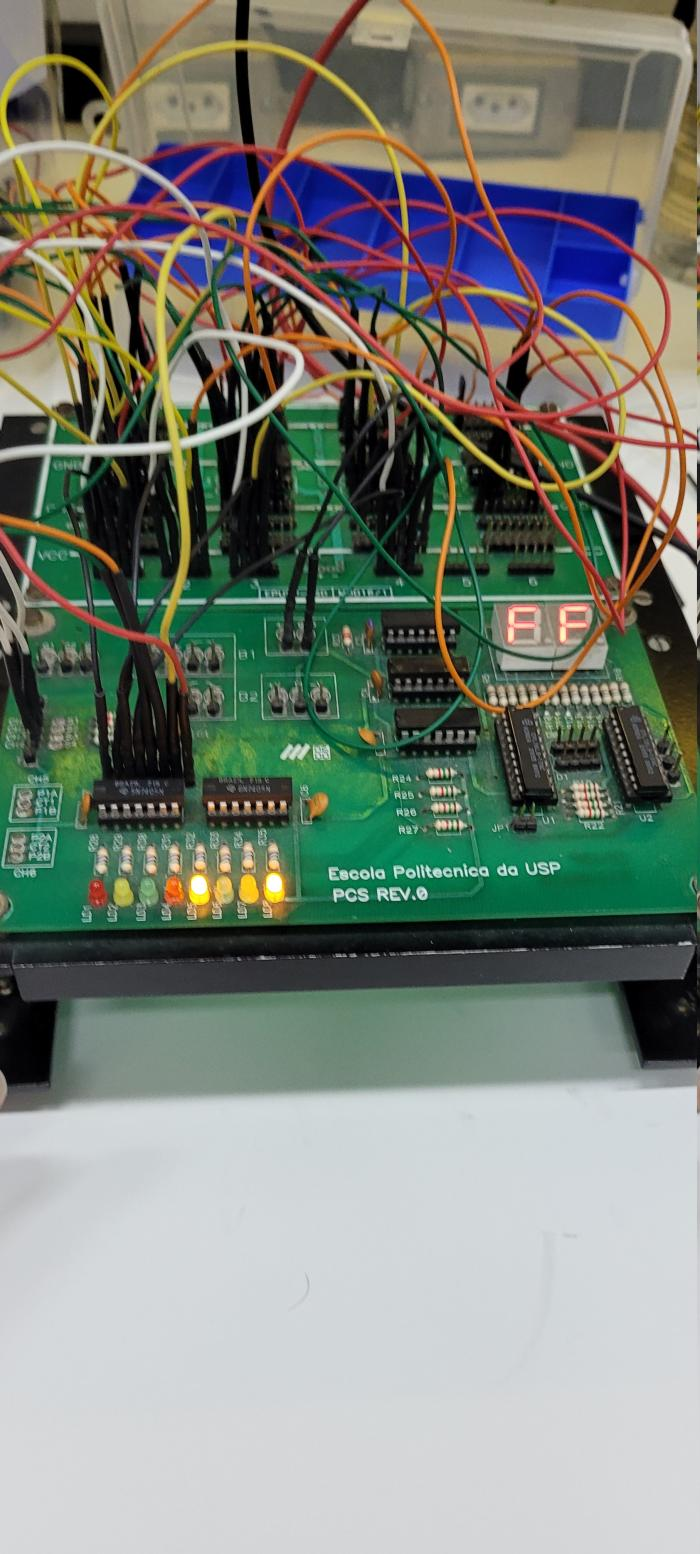
\includegraphics[width=0.45\textwidth, trim={0 20cm 0 7cm}, clip]{circ_1.jpg} & 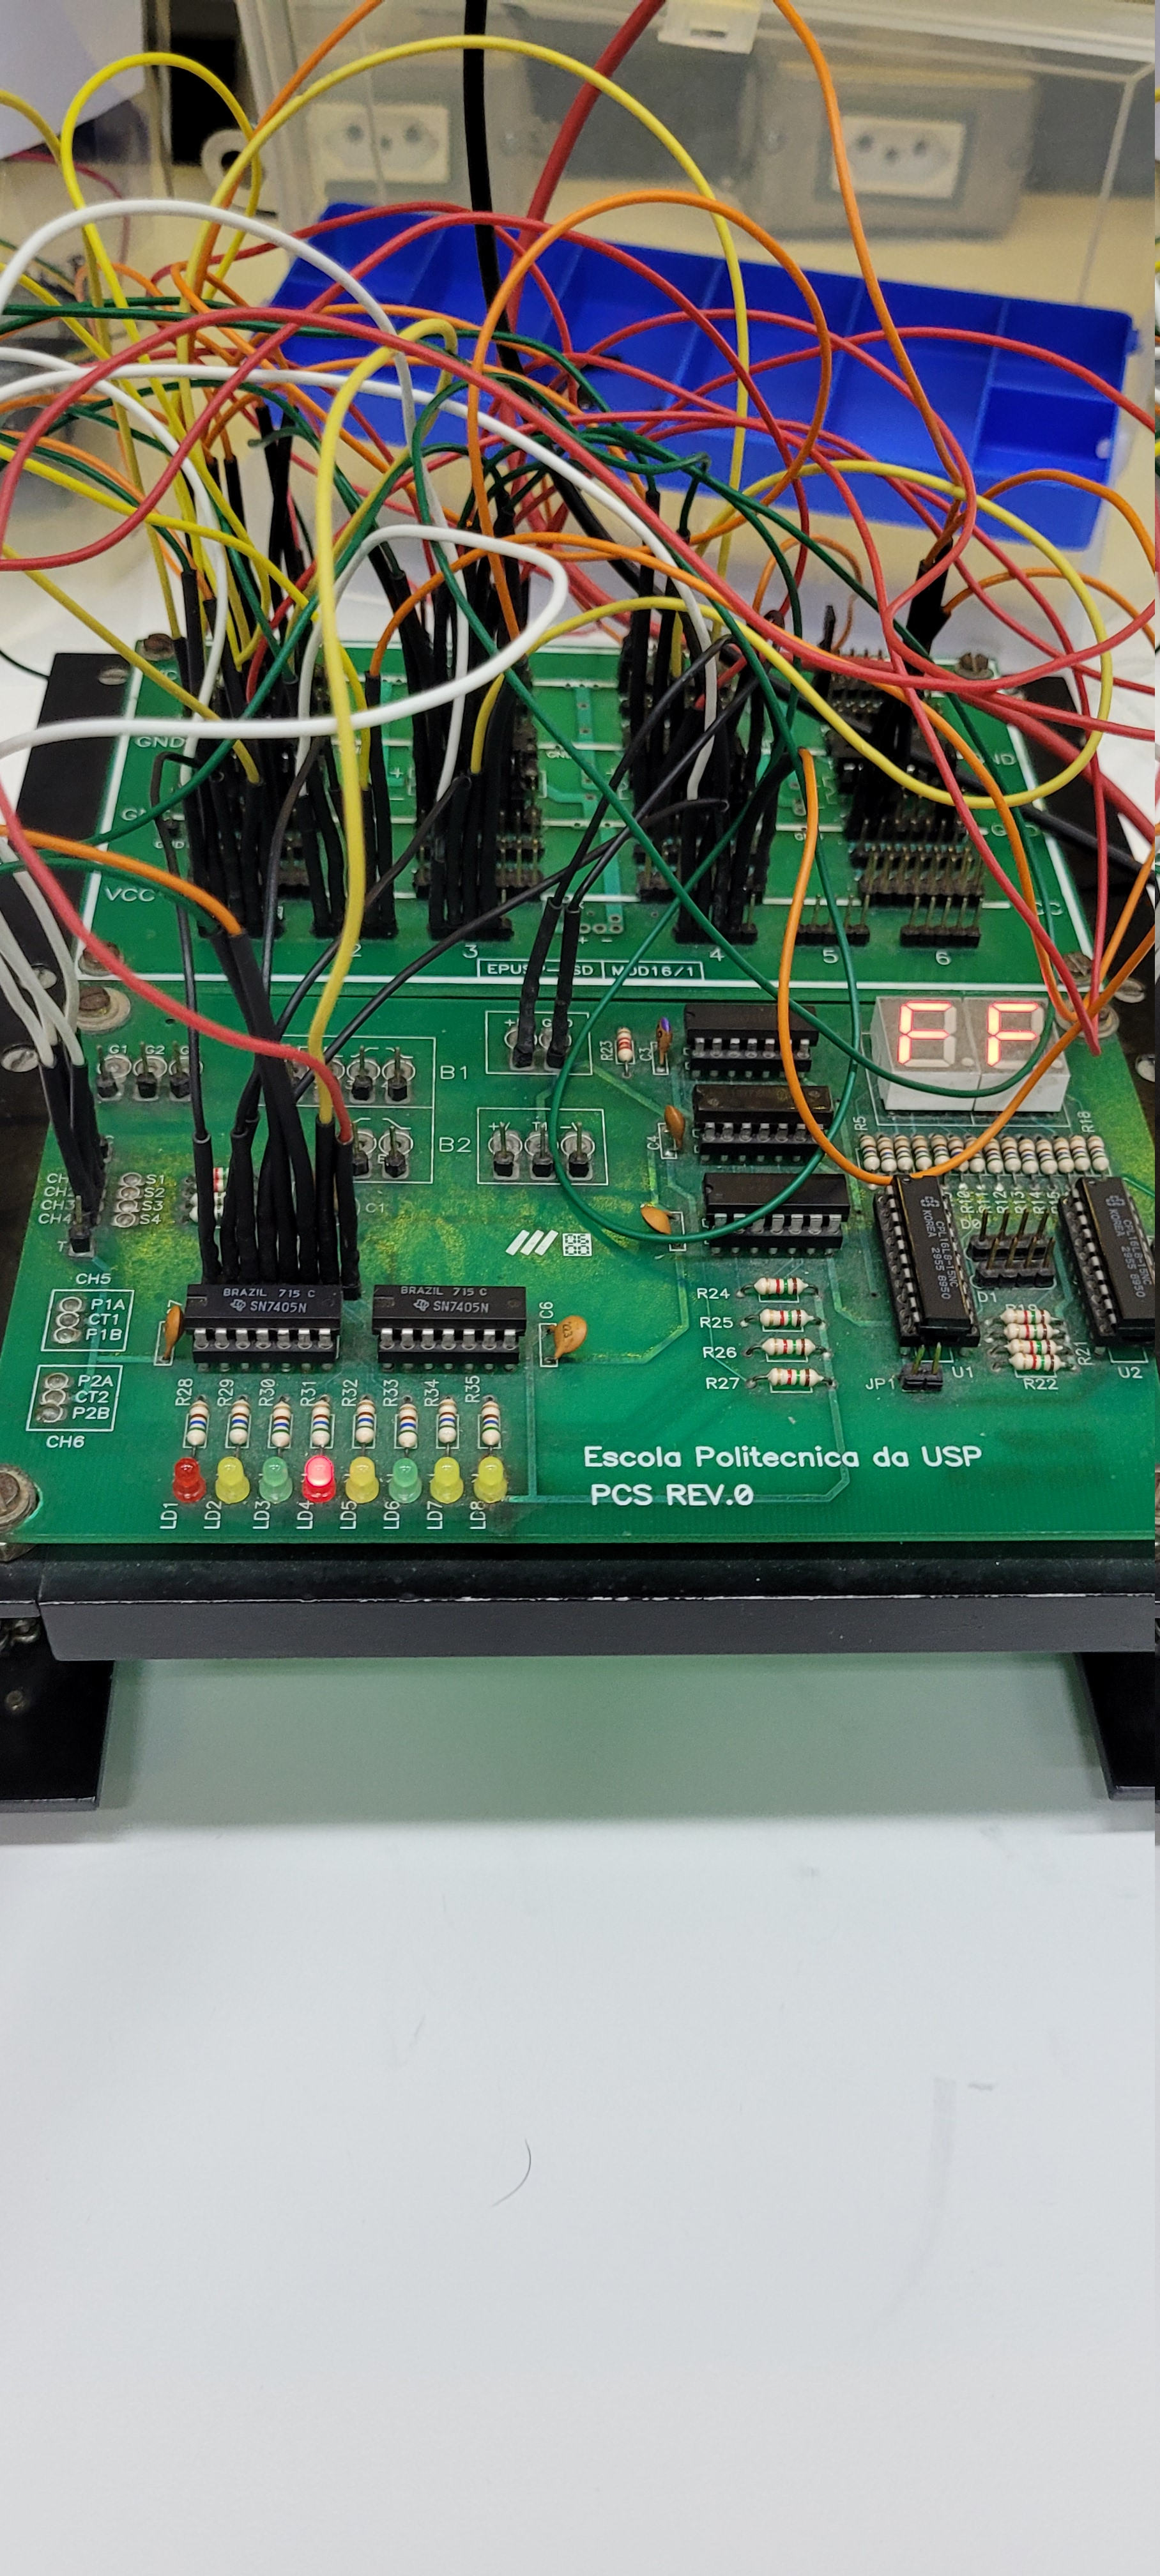
\includegraphics[width=0.45\textwidth, trim={0 20cm 0 7cm}, clip]{circ_2.jpg} \\
    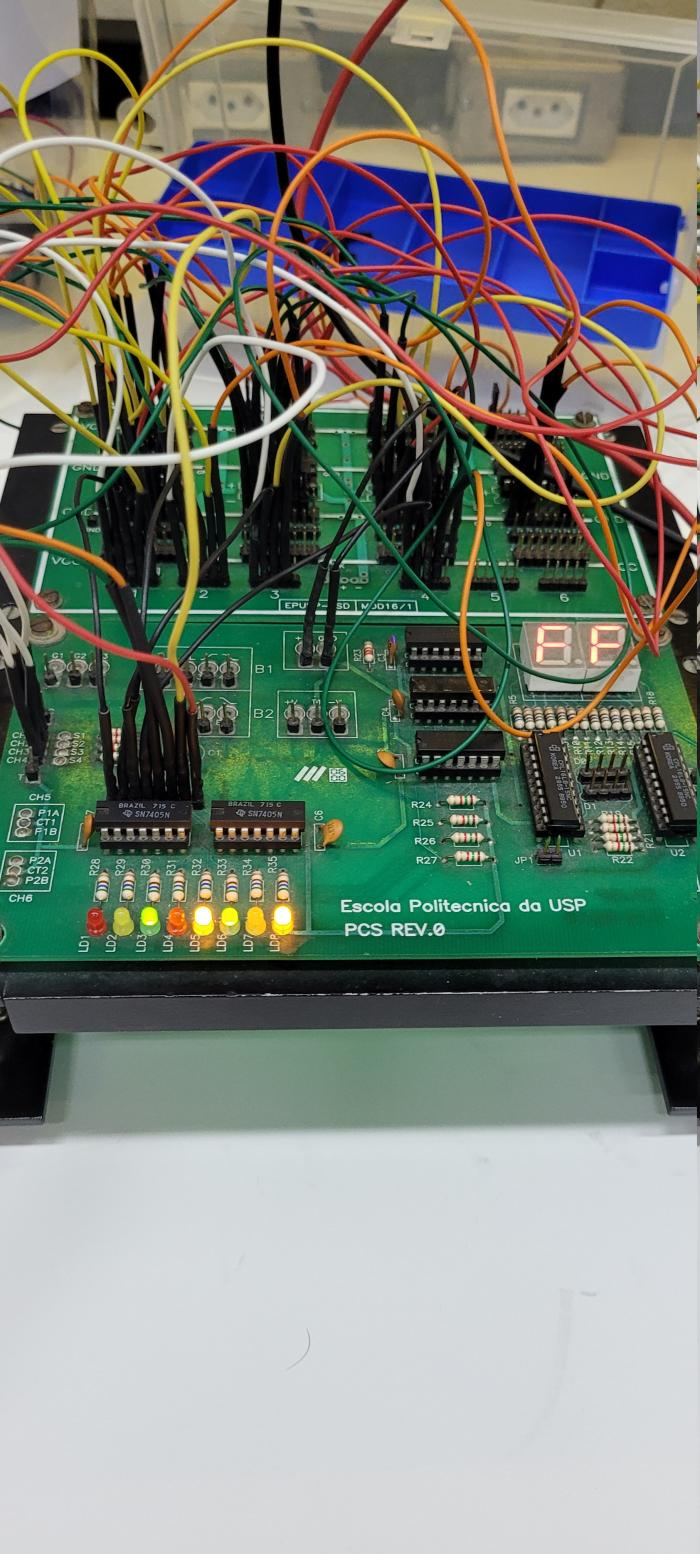
\includegraphics[width=0.45\textwidth, trim={0 18cm 0 7cm}, clip]{circ_3.jpg} & 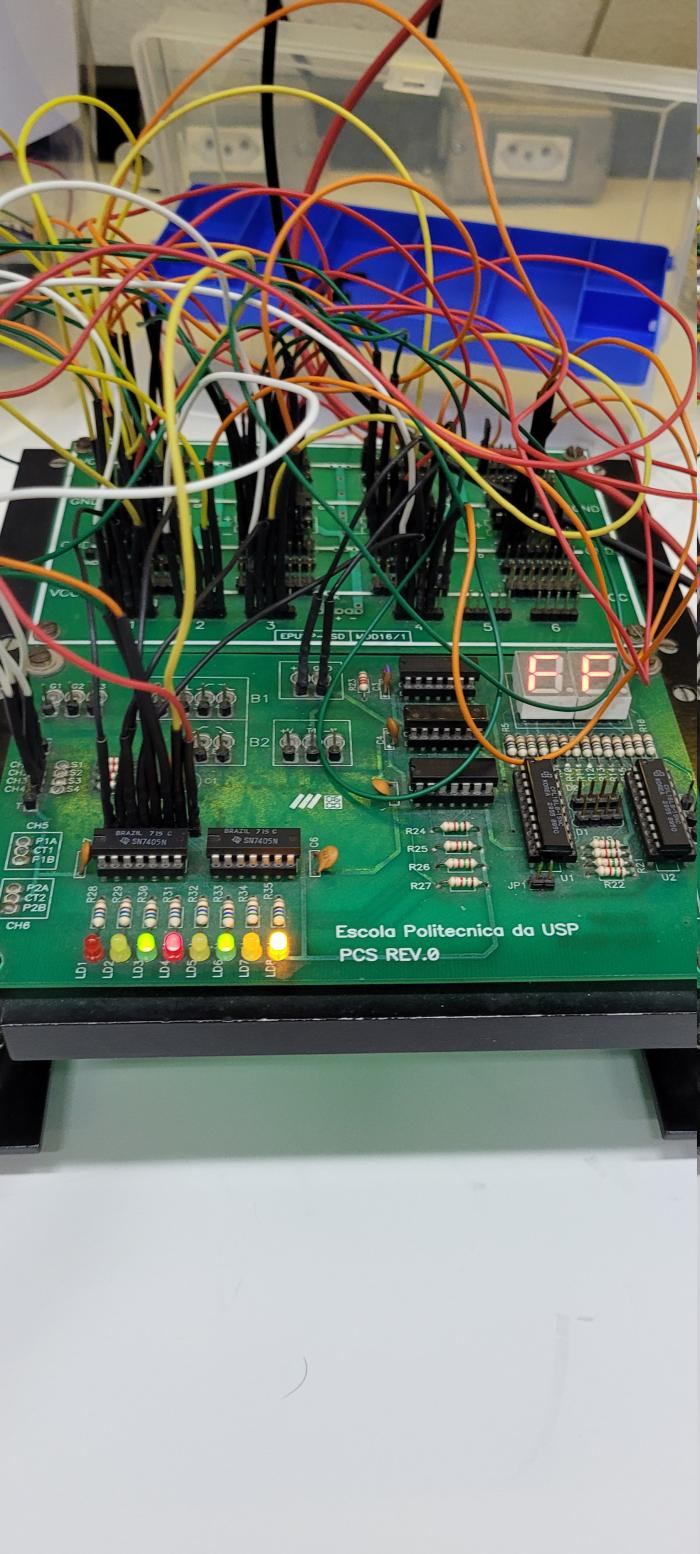
\includegraphics[width=0.45\textwidth, trim={0 18cm 0 7cm}, clip]{circ_4.jpg}
  \end{tabular}
  \caption{Montagem do circuito com os quatro primeiros valores, como mostra a Tabela Verdade experimental (Tabela \ref{tab:tabela_verdade_exp}).}
  \label{fig:montagem}
\end{figure}

\horizonBackCover
\end{document}
